\begin{center}
\begin{tikzpicture}
\begin{axis}[
    width=\dimexpr0.5\linewidth-1cm\relax,
    height=\dimexpr0.5\linewidth-1cm\relax,
    grid=both,
    unbounded coords=jump,
    title style={font=\small, yshift=0.6em},
    xlabel=$t$,
    ylabel style={%
        rotate=-90,
        anchor=east,
        overlay%
    },
    ylabel={$\varphi(t)=\dfrac{1}{1-\sin(t)}$},
    xmin=-6.5, xmax=6.5,
    ymin=-5, ymax=5,
    xtick={-6.283,-4.712,-3.141,-1.571,0,1.571,3.141,4.712,6.283},
    xticklabels={${}$,$-\frac{3\pi}{2}$,${}$,$-\frac{\pi}{2}$,${}$,$\frac{\pi}{2}$,${}$,$\frac{3\pi}{2}$,${}$}
]
\foreach \x in {-4.71, 1.571} {
  \addplot[dashed,gray,samples=2] coordinates {(\x,-5) (\x,5)};
}
\addplot[gray,thick,domain=-6.5:-4.71,samples=200,restrict y to domain=-5:5]
  {1/(1 - sin(deg(x)))};
\addplot[green!70!black,thick,domain=-4.71:1.57,samples=200,restrict y to domain=-5:6]
  {1/(1 - sin(deg(x)))};
\addplot[gray,thick,domain=1.57:6.5,samples=200,restrict y to domain=-5:5.1]
  {1/(1 - sin(deg(x)))};
\addplot[only marks, mark=*, mark size=1.5pt, green!70!black] coordinates {(0,1)};
\node[green!70!black] at (axis cs:0.3,0.3) {$(0,1)$};
\end{axis}
\end{tikzpicture}
\end{center}